\section{Concurrency Control}
\url{../other/professor's slides/2-ConcurrencyControl.pdf}\newline
\newline
The \textbf{concurrency control system}:
\begin{itemize}
    \item manage the simultaneous execution of transactions;
    \item avoids the insurgence of anomalies;
    \item ensure performance: exploit parallelism to maximise transactions per
    second.
\end{itemize}
\ \newline
Two transaction can have a \textbf{serial} execution, an \textbf{interleaved} execution or a \textbf{neasted} execution.
\begin{center}
    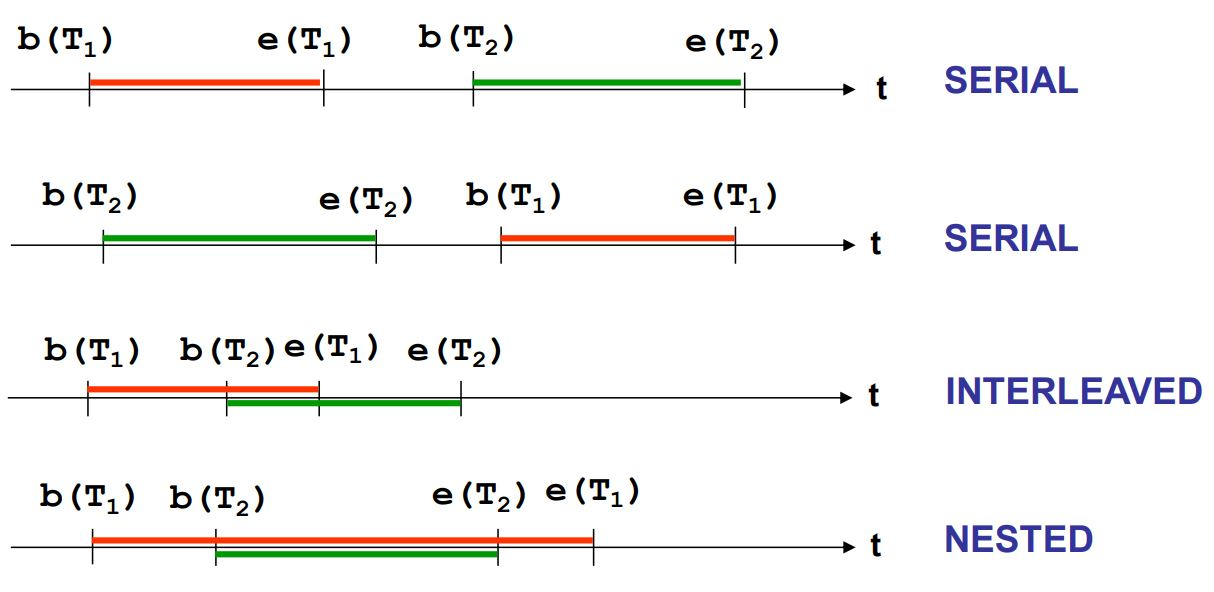
\includegraphics[height=4cm]{../arguments/serial-interleaved-nested.JPG}
\end{center}
\subsection{Anomalies}
An anomalie happens when two transaction are executed interleaved or nested and the result is different if they were executed serially.
\subsubsection{Lost Update}
\[
    r_1(x) \; \rightarrow \; r_2(x) \; \rightarrow \; w_1(x) \; \rightarrow \; w_2(x)
\]
An update is applied from a state that ignores a preceding update, wich is lost.
\subsubsection{Dirty Read}
\[
    r_1(x) \; \rightarrow \; w_1(x) \; \rightarrow \; r_2(x) \; \rightarrow \; abort_1 \; \rightarrow \; w_(2)
\]
An uncommitted (aborted transaction) value is used to update the data.
\subsubsection{Nonrepeatable Read}
\[
    r_1(x) \; \rightarrow \; r_2(x) \; \rightarrow \; w_2(x) \; \rightarrow \; r_1(x)
\]
Someone else updates a previously read value: inside of the same transaction a data is read and, after a while, without changing the value of the data, if we try to read it again, now its a different value.
\subsubsection{Phantom Update}
\[
    r_1(x) \; \rightarrow \; r_2(x) \; \rightarrow \; w_2(x) \; \rightarrow \; r_1(x)
\]
Someone else updates data that contributes to a previously read datum: a transaction reads multiple data, but at different times. There is inconcistency in the time of when the data that contributes to the constraints have been read.\newline
\newline
This anomaly is also known as "contraint violation".
\newline
Lets see an example: given the costraint $A+B+C = 100$ and the initial values $A = 50, B = 30, C = 20$\newline
$T_1 : r(A), r(B)$\newline
$T_2 : r(B), r(C)$\newline
$T_2 : $ subtract $10$ from $C$ and add $10$ to $B$.\newline
$T_2 : w(B), w(C)$\newline
$T_1 : r(C)$ ($T_1$ reads that the sum is $90$).\newline
So for $T_1$ it is as if "somebody else" had updated the value o the sum, but for $T_2$ the update is perfectly legal (does not change the value of the sum). 
\subsubsection{Phantom Insert}
\[
    r_1(x) \; \rightarrow \; w_2(new\; tuple) \; \rightarrow \; r_1(x)
\]
Someone else inserts data that contributes to a previously read datum.\newline
\newline
This anomaly does not depend on data already present in the DB when $T_1$ executes, but on a “phantom” tuple that is inserted by “someone else” and satisfies the conditions of a previous query of $T_1$.
\subsection{Principles of Concurrency Control}
\textbf{Operations}: a read or write of a specific datum by a specific transaction.\newline
\newline
\textbf{Schedule}: a sequence of operations performed by concurrent transactions that respects the order of operations of each transaction.\newline
How many distinct schedules exist for $n$ transaction each with $k_i$ operations?
\[
    N_D = \frac{\left(\sum_{i=1}^{n}k_i\right)!}{\Pi_{i=1}^n (k_i !)}
\]
How many of them are serial?
\[
    N_S = n!
\]
\ \newline
\textbf{Scheduler}: a component that accepts or rejects the operations requested by the transactions.\newline
\newline
\textbf{Serial schedule}: a schedule in which the actions of each transaction occur in a contiguos sequence.
\subsubsection{Serializable schedule}
A \textbf{serializable schedule} is a schedule that leaves the database in the \textbf{same state} as \textbf{some} serial schedule of the same transactions.
\begin{center}
    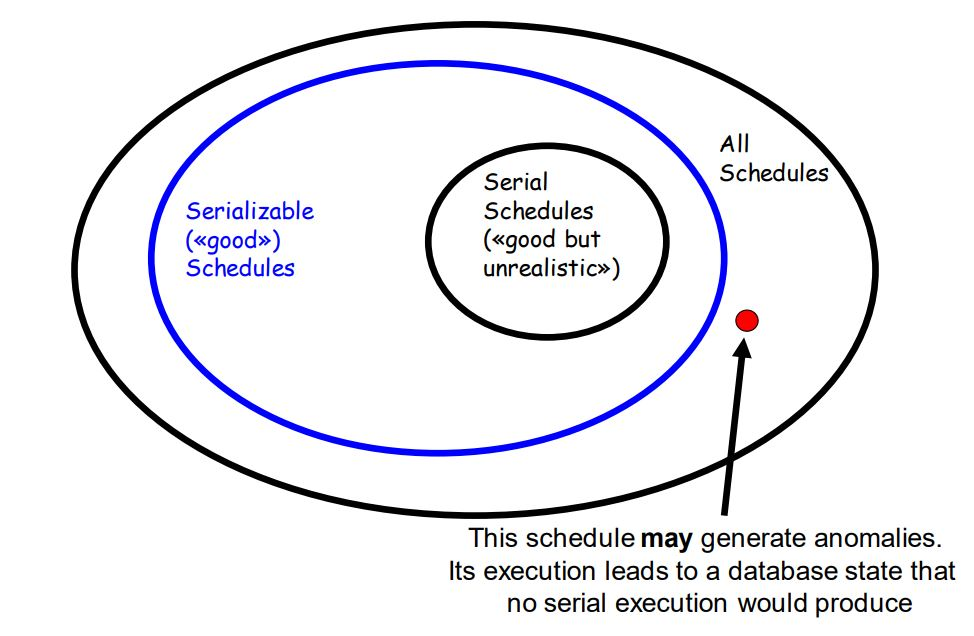
\includegraphics[height=6cm]{../arguments/serializableSchedules.JPG}
\end{center}
\subsubsection{View-serializability}
$r_i(x)$ \textbf{reads-from} $w_j(x)$ in a schedule $S$ when $w_j(x)$ precedes $r_i(x)$ and there is no $w_k(x)$ in $S$ between $r_i(x)$ and $w_j(x)$.\newline
\newline
$w_i(x)$ in a schedule $S$ is a \textbf{final write} if it is the last write on $x$ that occurs in $S$.\newline
\newline
Two schedules are \textbf{view-equivalent} if they have the same operations, the same reads-from relation, and the same final writes.\newline
\newline
A schedule is \textbf{view-serializable} if it is view-equivalent to a serial schedule of the same transactions.\newline
The class of view-serializable schedules is named \textbf{VSR}.\newline
$S$ is \textbf{view-serializable} if:
\begin{enumerate}
    \item every read operation sees the same values;
    \item the final value of each object is written by the same transaction as if the transactions were executed serially in some order.
\end{enumerate}
\ \newline
Deciding if a generic schedule is in VSR is an \textbf{NP-complete problem} but is an heavy task, so we look for a stricter definition that is easier to check, even if we reject sosme schedule that would be acceptable: VSR schedules are "too many".
\subsubsection{Conflict-serializability}
Two operations $o_i$ and $o_j$ are in \textbf{conflict} if they address the same resource and at least one of them is a write: \textbf{read-write} conflicts (r-w or w-r) and \textbf{write-write} conflicts (w-w).\newline
\newline
Two schedules are \textbf{conflict-equivalent} if contain the same operations and in all conflicting pairs transactions occur in the same order.\newline
\newline
A schedule is \textbf{conflict-serializable} if it is conflict-equivalent to a serial schedule of the same transactions.\newline
The class of conflict-serializable schedules is named \textbf{CSR}.
\newline
\newline
All conflict-serializable schedules are also view-serializable, but the inverse is not necessarily true: $CSR \rightarrow VSR$.
\begin{center}
    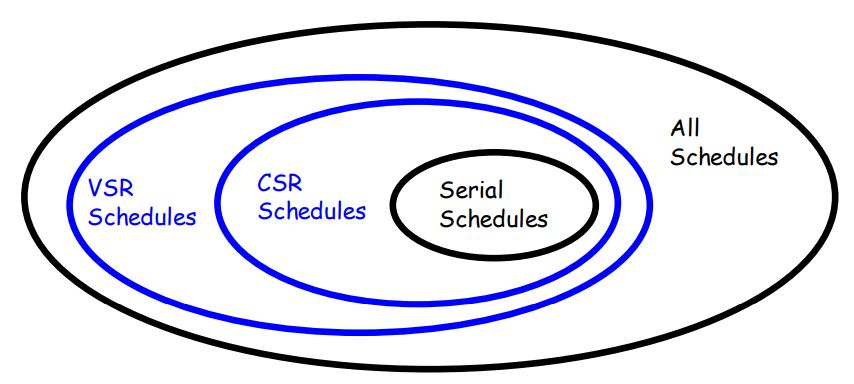
\includegraphics[height=5cm]{../arguments/CSRandVSR.JPG}
\end{center}
\subsubsection{Testing conflict-serializability}
To check if a schedule is conflict-serializable we use a \textbf{conflict graph}:
\begin{itemize}
    \item one node for each transaction $T_i$;
    \item one arc from $T_i$ to $T_j$ if there exists at least one conflict between an operation $o_i$ of $T_i$ and an operations $o_j$ of $T_j$ such that $o_i$ precedes $o_j$;
    \item a schedule is in CSR if and only if its conflict graph is \textbf{acyclic}.
\end{itemize}
To check if a graph is acyclic we use this algorithm:
\begin{itemize}
    \item if a graph is acyclic, then it must have at least one node with no targets, called leaf (with no arrows going away from the node).
    \item if we "peel off" a leaf in an acyclic graph, then we are always left with an acyclic graph, and if we keep peeling off leaf nodes, one of two things will happen: we will eventually peel off al node and so the graph is acyclic, or we will get to a point where there is no leaf, yet the graph is not empty and so the graph is cyclic.
\end{itemize}
If $S$’s graph is acyclic then it induces a \textbf{topological (partial) ordering} on its nodes, that is easier to understand graphically with an example:
\begin{center}
    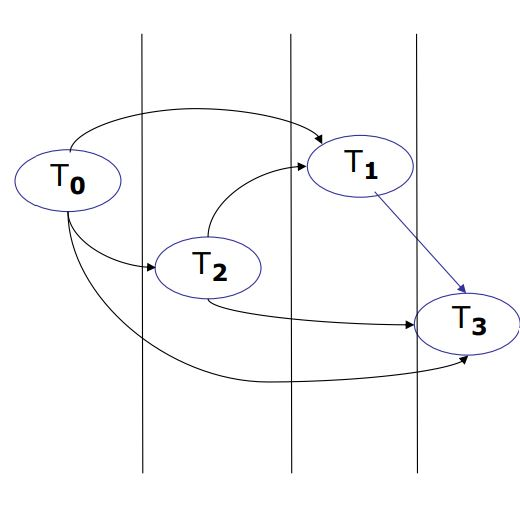
\includegraphics[height=5cm]{../arguments/topologicalpartialorderingCSR.JPG}
\end{center}
In general, there can be many compatible serial schedules.
\subsection{Concurrency control based on locking}
Everything we have seen untill now is based on study of schedules after they have been executed. In real life we need a system that can assure cocnurrency control in "live".\newline
There are two main families of techniques:
\begin{itemize}
    \item Pessimistic: based on locks, resource access control.
    \item Optimistic: based on timestamps and versions, serve as many requests as possible, possibly using out-of-date versions of the data.
\end{itemize}
\subsubsection{Locking}
A transaction is \textbf{well-formed w.r.t. locking} if
\begin{itemize}
    \item read operations are preceded by \textbf{r\_lock} (shared lock SL) and followed by \textbf{unlock};
    \item write operations are preceded by \textbf{w\_lock} (exclusice lock XL) and followed by \textbf{unlock}.
\end{itemize}
\ \newline
Transactions that first read and then write an object may:
\begin{itemize}
    \item acquire a w\_lock already when reading or
    \item acquire a r\_lock first and then upgrade it into a w\_lock (lock \textbf{escalation}).
\end{itemize}
\ \newline
Possible states of an object:
\begin{itemize}
    \item \textbf{free};
    \item \textbf{r-locked} (locked by one or more readers);
    \item \textbf{w-locked} (locked by a writer);
\end{itemize}
\ \newline
When a lock request is granted, the resource is acquired; when an unlock is executed, the resource becomes available.\newline
The lock manager grants access to resources according to the \textbf{conflict table}:
\renewcommand{\arraystretch}{1.5}
\begin{center}
    \begin{tabular}{ |c|c c c| } 
     \hline
     & FREE & R\_LOCKED & W\_LOCKED \\ 
     \hline
     r\_lock & \textcolor{green}{OK} (R\_LOCKED) & \textcolor{green}{OK} (R\_LOCKED n++) & \textcolor{red}{NO} (W\_LOCKED) \\ 
     w\_lock & \textcolor{green}{OK} (W\_LOCKED) & \textcolor{red}{NO} (R\_LOCKED) & \textcolor{red}{NO} (W\_LOCKED)\\ 
     unlock & \textcolor{red}{ERROR} & \textcolor{green}{OK} (DEPENDS n- -) & \textcolor{green}{OK} (FREE) \\ 
     \hline
    \end{tabular}
\end{center}
\renewcommand{\arraystretch}{1}
where $n$ is the counter of the current readers.
\subsubsection{2PL}
Is respecting locks enough for serializability? No. For example non repeatable read anomalies can still occur and to prevent it we use the \textbf{Two-Phase Locking (2PL)}: the requirement (two-phase rule) is that \textbf{"a transaction cannot acquire any other lock after releasing a lock"}. Doing so we prevent \textbf{non repeatable reads}.\newline
\newline
A scheduler that only processes well-formed transactions, grants locks according to the conflict table and checks that all transactions apply the two-phase rule generetes a class of schedules called \textbf{2PL}.\newline
\newline
\textbf{Schedules in 2PL are view- and conflict-serializable}. 2PL impies CSR.
\begin{center}
    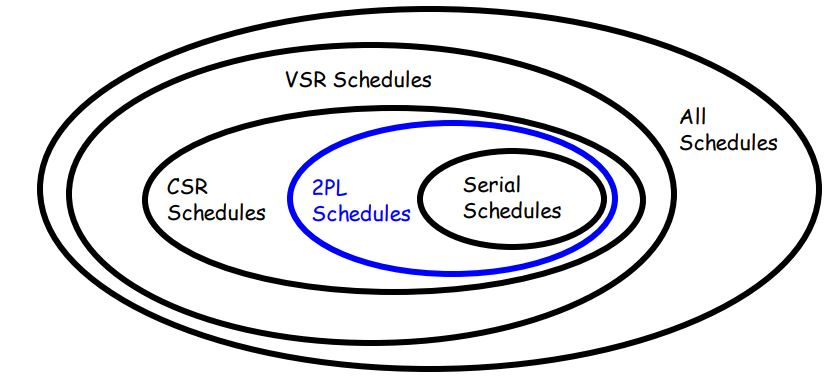
\includegraphics[height=5cm]{../arguments/2PL.JPG}
\end{center}
\subsubsection{Strict 2PL}
Up to now, we were still using the \textbf{hypothesis of
commit-projection} (no transactions in the schedule
abort).\newline
2PL, as seen so far, does not protect against \textbf{dirty} (uncommitted data) \textbf{reads} (and therefore neither do VSR nor CSR): releasing locks before rollbacks exposes “dirty” data.\newline
\newline
To remove this hypothesis, we need to add a constraint to
2PL, that defines \textbf{strict 2PL}: \textbf{Locks held by a transaction can be released only after
commit/rollback}.\newline
\newline
Strict 2PL locks are also called \textbf{long duration locks}, 2PL locks \textbf{short duration locks}.\newline
\newline
A phantom insertion occurs when a transaction adds items to a data set previously read by another transaction. To prevent phantom inserts a lock should be placed also on
“future data”.\newline
\newline
\textbf{Predicate locks} extend the notion of \textbf{data locks} to “future data”. Predicate locks are a tool to lock data that doesn't already exist.\newline
\newline
Write locks are held until the completion (commit) of the transaction, and not only untill the end of the write, to enable the proper processing of abort events.\newline
\newline
\newline
2PL and locking have two foundamentals principles:
\begin{itemize}
    \item \textbf{same transaction i}: a transaction consists of a growing phase (locking resources), a plateau (operations) and a shrinking phase (releasing locks). Because of the 2PL rule we can say that all the locks must happen before the unlocks:
    \[
        L^?_i < U^?_i
    \]
    \item \textbf{same resource R}: if we analyze a resource, we can say that before being able to lock a resource, it must be unlocked by the precedent transaction that was locking it:
    \[
        U^R_? < L^R_?
    \]
    this constraint is not a 2PL rule, but is necessary to have a working locking system.
\end{itemize}
\subsubsection{Isolation Levels in SQL:1999 (and JDBC)}
Isolation Levels in SQL:1999 (and JDBC):
\begin{itemize}
    \item READ UNCOMMITTED allows dirty reads, nonrepeatable reads and
    phantom updates and inserts: No read locks (and ignores locks of other transactions).
    \item READ COMMITTED prevents dirty reads but allows nonrepeatable
    reads and phantom updates/inserts: Read locks (and complies with locks of other transactions), but
    without 2PL on read locks (read locks are released as soon as
    the read operation is performed and can be acquired again).
    \item REPEATABLE READ avoids dirty reads, nonrepeatable reads and
    phantom updates, but allows phantom inserts: long duration read locks $\rightarrow$ 2PL also for reads.
    \item SERIALIZABLE avoids all anomalies: 2PL with predicate locks to avoid phantom inserts
\end{itemize}
\ \newline
The locking requirements to meet this guarantee can
frequently lead to deadlock where one of the transactions
needs to be rolled back. Therefore SERIALIZABLE isolation level is used sparingly and
is NOT the default in most commercial systems.
\newline
\newline
SQL Isolation levels may be implemented with the appropriate
use of lock.\newline
The isolatioon levels define the way read lock are managed, write lock are always managed in strict 2PL (because it is the only way to handle aborts).
\begin{center}
    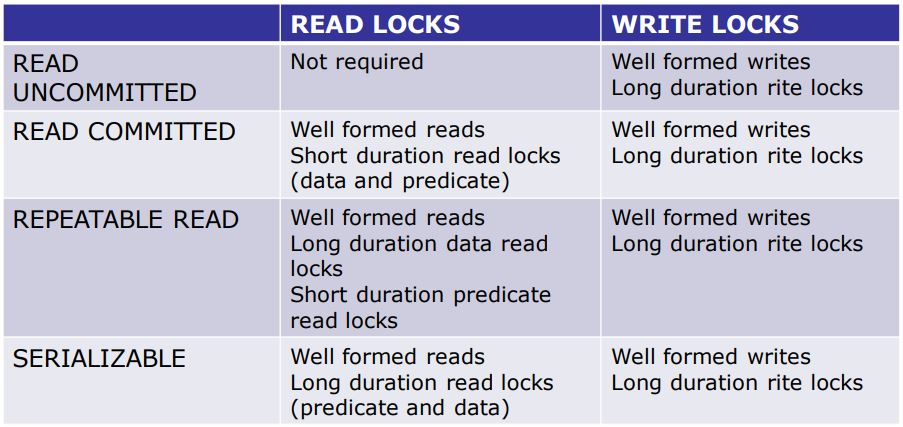
\includegraphics[height=5cm]{../arguments/isolationlevels.JPG}
\end{center}
\subsubsection{Deadlock}
A resource can be free, read-locked or write-locked.\newline
\newline
Transactions requesting locks are either \textbf{granted the lock} or
\textbf{suspended and queued} (first-in first-out). There is risk of:
\begin{itemize}
    \item \textbf{deadlock}: two or more transactions in endless (mutual) wait (Typically occurs when each transaction waits for
    another to release a lock).    
    \item \textbf{starvation}: a single transaction in endless wait (Typically occurs due to write transactions waiting for
    resources that are continuously read).
\end{itemize}
\ \newline
\textbf{Lock graph}:  a bipartite graph in which nodes are resources
or transactions and arcs are lock requests or lock
assignments.\newline
\newline
\textbf{Wait for graph}:  a graph in which nodes are transactions
and arcs are “waits for” relationships.\newline
A deadlock is represented by a cycle in the wait-for graph
of transactions.\newline
\newline
Deadlock resolution techniques:
\begin{itemize}
    \item \textbf{Timeout}: transaction killed and restarted after a given
    amount of waiting;
    \item \textbf{Deadlock prevention}: transaction killed when they could be in deadlock.
    \begin{itemize}
        \item \textbf{Resource-based prevention}: transactions request all resources at once, and only once; resources are globally sorted and must be requested in that order.
        \item \textbf{Transaction-based prevention}: assigning IDs to transactions incrementally (transactions' "age") and preventing older transactions from waiting for younger ones to end their work.
    \end{itemize}
    \item \textbf{Deadlock detection}: transaction killed when they are in deadlock. Requires an algorithm to detect cycles in the wait-for graph.
\end{itemize}
\subsubsection{Deadlock detection}
The deadlock detectiton requires an algorithm to detect cycles in the wait-for graph.\newline
\newline
Assumptions:
\begin{itemize}
    \item Transactions execute on a single main node (one locus of
    control);
    \item Transactions may be decomposed in “sub-transactions”
    running on other nodes;
    \item Synchronicity: when a transaction spawns a sub-transaction it
    suspends work until the latter completes;
    \item Two waits-for relationships: (1) $T_i$ waits from $T_j$ on the same node because $T_i$ needs a datum locked by $T_j$; (2) a sub-transaction of $T_i$ waits for another sub-transaction of $T_i$ running on a different node.
\end{itemize}
Because of the macanism of sub-transactions we need a distributed dependency graph, that is a global view of all the dependencies in all the differents nodes, where external call nodes represent a sub-transaction activating another sub-transaction at a different node.\newline
\newline
We will use the symbol "$\rightarrow$" as a "wait for" relation among local transactions.\newline
\newline
Lets see an example of deadlock (cycle) in a distributed dependency graph:
\begin{center}
    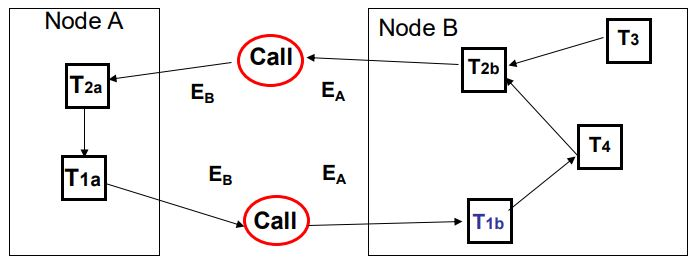
\includegraphics[height=5cm]{../arguments/distributeddependencygraph.JPG}
\end{center}
We can see a cycle between two differents node (A and B) in $T_{2a} \rightarrow T_{1a} \rightarrow T_{1b} \rightarrow T_{2b} \rightarrow T_{2a}$.\newline
\newline
The problem is how we can detect such occurance without maintaining the global view of the distributed dependeny graph but keeping it as much possible local for each node. To do so we need to  establish a communication protocol whereby each node has a local projection of the global dependencies. Nodes exchange information and update their local graph based on the received information and communication is optimized to avoid that multiple nodes detect the same potential deadlock.\newline
\newline
Node $A$ sends its local info to a node $B$ only if
\begin{itemize}
    \item $A$ contains a transaction $T_i$ that is waited from another remote transaction and waits for a transaction $T_j$ active on $B$;
    \item $i>j$ (this ensure a kind of message "forwarding" along a node path where node $A$ "precedes" node $B$ if $i>j$).
\end{itemize}
Mnemonically: I send info to you if a d-transaction listed at me waits for a d-transaction listed at you with smaller index.
\subsubsection{Obermark's algorithm}
The Obermark's algorithm runs periodically at each node and consists of four steps:
\begin{itemize}
    \item Get graph info (wait dependencies among transactions
    and external calls) from the "previous" nodes.
    Sequences contain only node and top-level transaction
    identifiers
    \item Update the local graph by merging the received
    information
    \item Check the existence of cycles among transactions
    denoting potential deadlocks: if found, select one
    transaction in the cycle and kill it
    \item Send updated graph info to the “next” nodes
\end{itemize}
\subsubsection{Update lock}
The most frequent deadlock occurs when two concurrent
transactions start by reading the same resources (SL) and
then decide to write and try to upgrade their lock to write (XL).\newline
\newline
To avoid this situation, systems offer the \textbf{update lock} (UL): is a special lock asked by transactions that will read and then write an item..\newline
\newline
Here it is the \textbf{table of conflict} with the update lock:
\renewcommand{\arraystretch}{1.5}
\begin{center}
    \begin{tabular}{ |c|c c c| } 
     \hline
      & & resource status & \\
     request & SL & UL & XL \\ 
     \hline
     SL & \textcolor{green}{OK} & \textcolor{green}{OK} & \textcolor{red}{NO} \\ 
     UL & \textcolor{green}{OK} & \textcolor{red}{NO} & \textcolor{red}{NO} \\ 
     XL & \textcolor{red}{NO} & \textcolor{red}{NO} & \textcolor{red}{NO} \\ 
     \hline
    \end{tabular}
\end{center}
\renewcommand{\arraystretch}{1}
\ \newline
The price for using update locks is that they extend the interval during which a resource is locked.
\subsubsection{Hierarchical locking}
Locks can be specified with different granularities (schema, table, fragment, page, tuple, field) and we have two objectives: locking the minimum amount of data and recognizing conflicts as soon as possible. We obtain this by requesting resources top-down until the right level is obtained and releasing locks bottom-up.\newline
\newline
The \textbf{intention locking scheme} is a mode to express the intention of locking at lower levels of granularity, there are 3 more lock modes in addition to SL (read shared locks) and XL (write exclusive locks):
\begin{itemize}
    \item \textbf{ISL}: Intention of locking a subelement of current element
    in shared mode
    \item \textbf{IXL}: Intention of locking a subelement of current
    element in exclusive mode
    \item \textbf{SIXL}: Lock of the element in shared mode with intention
    of locking a subelement in exclusive mode (SL+IXL)    
\end{itemize}
\textbf{Hierarchical locking}:
\begin{itemize}
    \item Locks are requested starting from the root (the whole table) and going down in the hierarchy;
    \item Locks are released starting from the leaves and going up
    in the hierarchy
    \item To request an SL or ISL lock on a non-root element, a
    transaction must hold an equally or more restrictive lock
    (ISL or IXL) on its "parent"
    \item  To request an IXL, XL or SIXL lock on a non-root element,
    a transaction must hold an equally or more restrictive lock
    (SIXL or IXL) on its "parent"
    \item When a lock is requested on a resource, the lock manager
    decides based on the rules specified in the hierarchical
    lock granting table 
\end{itemize}
\textbf{Hierarchical lock granting table}:
\begin{center}
    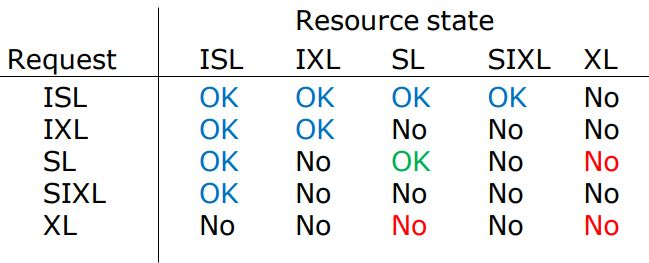
\includegraphics[height=4cm]{../arguments/hierarchicallockgrantingtable.JPG}
\end{center}
\subsection{Concurrency control based on timestamps}
Locking is also named pessimistic concurrency control because it assumes that collisions will arise, alternative are the optimistic concurrency control methods like concurrency control based on timestamps.\newline
\newline
\textbf{Timestamp}: Identifier that defines a total ordering of events of a system.\newline
\newline
Each transaction has a timestamp representing the time
at which the transaction begins so that transactions can
be ordered by “birth date”.
\subsubsection{Timestamps in distributed systems}
How do we assign timestamps in distributed systems where there is no "global time" available? A system’s function gives out timestamps on requests.\newline
We can now use an algorithm, known as "Lamport method": cannot receive a message from "the
future", if this happens the "bumping rule" is used to bump the
timestamp of the receive event beyond the timestamp of the send
event.\newline
\newline
Mnemonically: if I receive a message from you that has a
timestamp greater than my last emitted one I update my current
timestamp to exceed yours.
\subsubsection{Timestamp principles}
The scheduler has two counters: RTM(x) and WTM(x) for each object.\newline
\newline
The scheduler receives read/write requests tagged with timestamps:
\begin{itemize}
    \item read(x,ts): if ts $<$ WTM(x) the request is rejected and the transaction is killed, else access is granted and RTM(x) is set to max(RTM(x),ts);
    \item write(x,ts): if ts $<$ RTM(x) or ts $<$ WTM(x) the request is rejected and the transaction is killed, else access is granted and WTM(x) is set to ts.
\end{itemize}
This approach uses a commit-projection hypothesis, meaning that there are no abort and each transaction is committed.\newline
To work without this hypothesis write operations should be buffered until commit, in this way aborted transactions do not even issue write requests and the commit-projection hypothesis is equivalent to a full schedule with committed and abored transactions.
\begin{center}
    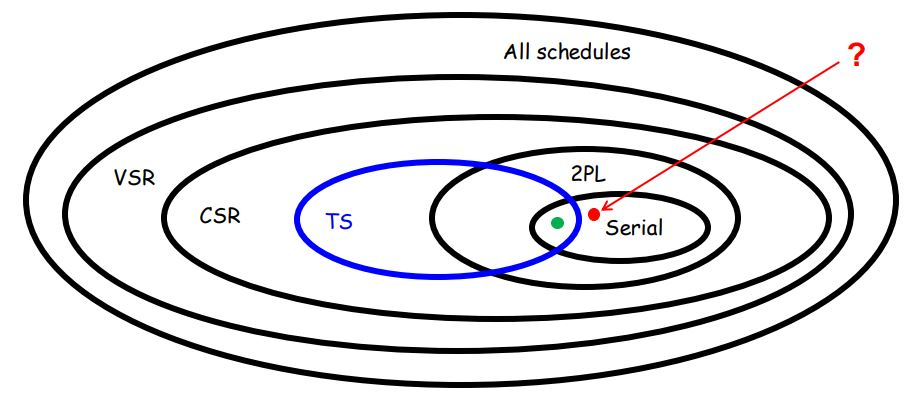
\includegraphics[height=5cm]{../arguments/tsand2pl.JPG}
\end{center}
Notice how some serial transaction aren't present in the timestamp approach.\newline
\newline
In 2PL transactions can be actively waiting. In TS they are
killed and restarted. Restarting a transaction costs more than waiting: 2PL wins!
\subsubsection{Thomas Rule}
A variant of the basic timestamp-based concurrency control is the Thomas Rule, where the only thing that change is the write(x,ts) rule:
\begin{itemize}
    \item if ts $<$ RTM(x) the request is rejected and the transaction is killed, else if ts $<$ WTM(x) then our write is "obsolete": it can be skipped.
\end{itemize}
Skipping a write on an object that has already been written
by a younger transaction, without killing the transaction, works only if the transaction issues a write without requiring a previous
read on the object (so SET X = X+1 would fail).
\begin{center}
    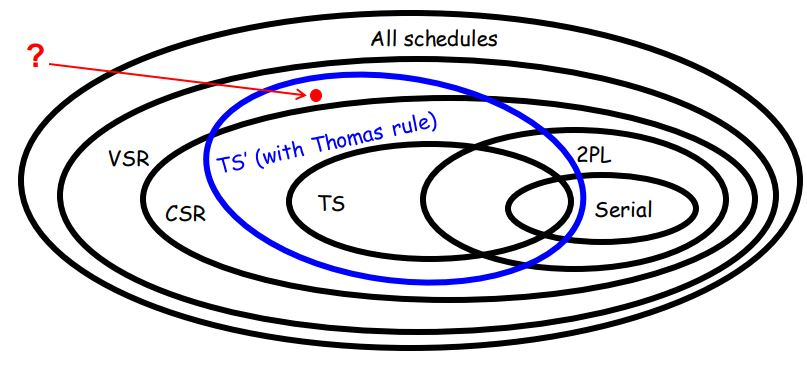
\includegraphics[height=5cm]{../arguments/thomasrule.JPG}
\end{center}
\subsubsection{Multiversion concurrency control}
Idea: writes generate new copies, reads access the
"right" copy.\newline
\newline
Writes generate new copies, each one with a new WTM.
Each object x always has n$>=$1 active copies with
WTMn(x). There is a unique global RTM(x).\newline
\newline
Old copies are discarded when there are no
transactions that need these values.
\newline
\newline
Mechanism:
\begin{itemize}
    \item read(x,ts): is always accepted, a copy $x_k$ is selected for reading such that if ts $>$ WTMn(x), then k = n, else take $k$ sucj that WTMk(x) $\leq$ ts $< WTM_{k+1}(x)$. 
    \item write(x,ts): if ts $<$ RTM(x) the request is rejected, else a new version is created (n is incremented) with WTMn(x) = ts.
\end{itemize}
\begin{center}
    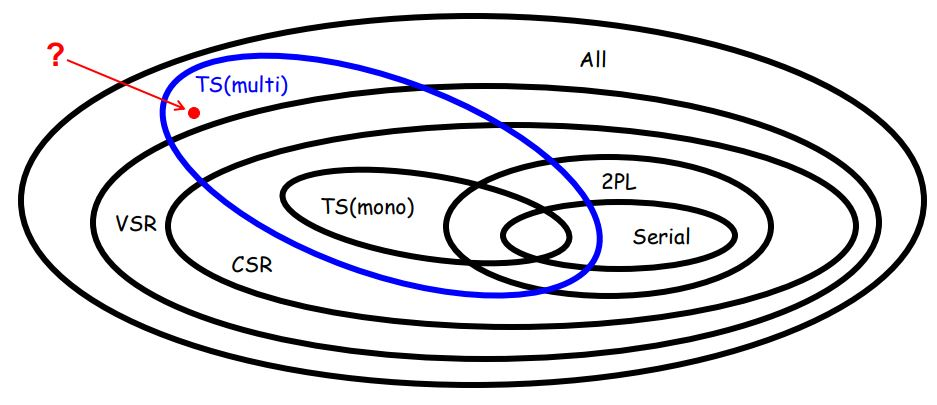
\includegraphics[height=5cm]{../arguments/multiversionts.JPG}
\end{center}